%-------------------------------------------------------
\section{How Do We Know Things?}
\subsection{Locke}
%-------------------------------------------------------
\begin{frame}{How Do We \textit{Know} Things?}{Locke}
%-------------------------------------------------------

	\begin{columns}[T]
		\column{0.5\textwidth}
		Locke was an English, Protestant philosopher who created the foundations for empiricism. He divided human thought into two categories:
		\begin{enumerate}
			\item Knowledge
			\item Belief
		\end{enumerate}
		This difference between what is known and what is believed was a great influence on Thomas Jefferson. In fact, Jefferson called Locke "[one] of the greatest men the world had ever produced"
		\column{0.5\textwidth}
		\begin{figure}
			\centering
			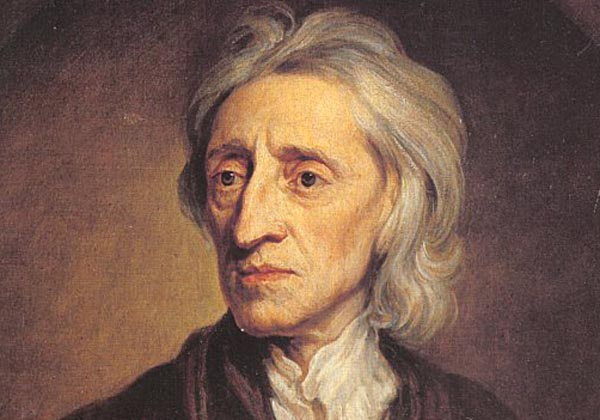
\includegraphics[width=\textwidth]{images/locke.jpg}
			\caption{John Locke}
		\end{figure}
	\end{columns}

 \end{frame}

%-------------------------------------------------------
\subsection{Knowledge}
%-------------------------------------------------------
\begin{frame}{How Do We \textit{Know} Things?}{Knowledge}
%-------------------------------------------------------

	\begin{columns}[T]
		\column{0.5\textwidth}
		Knowledge - which itself he divided into three distinct types
		\begin{itemize}
			\item Intuitive - Knowledge which is "self-evident"; "common sense"
			\item Demonstrative - Knowledge which can be shown to be true using a rigorous list of steps in reasoning (called "proofs")
			\item Sensitive - Knowledge which is gained from observing the world.%\\
		\end{itemize}
		\column{0.5\textwidth}
		\begin{figure}
			\centering
			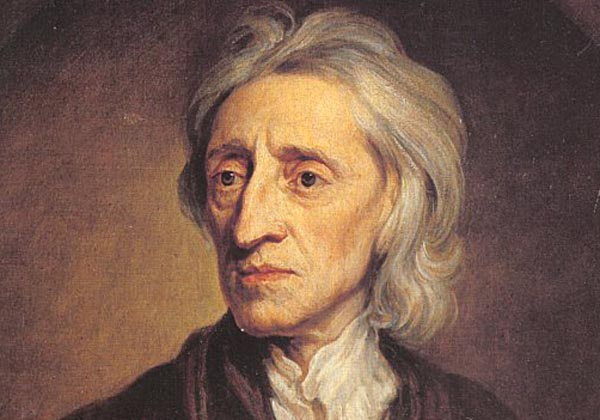
\includegraphics[width=\textwidth]{images/locke.jpg}
			\caption{John Locke}
		\end{figure}
	\end{columns}

 \end{frame}
